\section{Superconducting Magnet}
When designing a particle detector choice of magnet configuration drives
much of the detector layout and design; large bending power is required to precisely 
measure the momentum of high-energy charged particles. This forced the CMS
collaboration to choose superconducting technology for the magnets.
The superconducting solenoid magnet used in CMS was designed to reach a 4-T field;
during the 2011 and 2012 runs it was operated at a central magnetic flux
density of 3.8-T to reduce the effects of aging on the coil. %%%Cite http://iopscience.iop.org/1748-0221/5/03/T03021/pdf/1748-0221_5_03_T03021.pdf
The purpose of this magnetic field is to allow precise measurement of the 
momentum of charged particles, across a wide range of energies, originating from LHC collisions. 

For a charged particle in a uniform magnetic field the  momentum of the charged particle is given by,
\begin{displaymath}
p=qBr
\end{displaymath}  
Where p is the momentum of the particle, q is its charge, B is the 
magnetic field strength and r is the radius of the particle's trajectory.
The transverse momentum resolution depends on the magnetic field and
solenoid radius as
\begin{displaymath}
\frac{dp}{p}\propto\frac{p}{BL^{2}}
\end{displaymath}
%Therefore, 
%is used for the measurement of track momenta in the tracker 
%and to predict track bendin
%by reconstructing the path of charged particle in the tracker
\begin{figure}[hb]
  \centering
	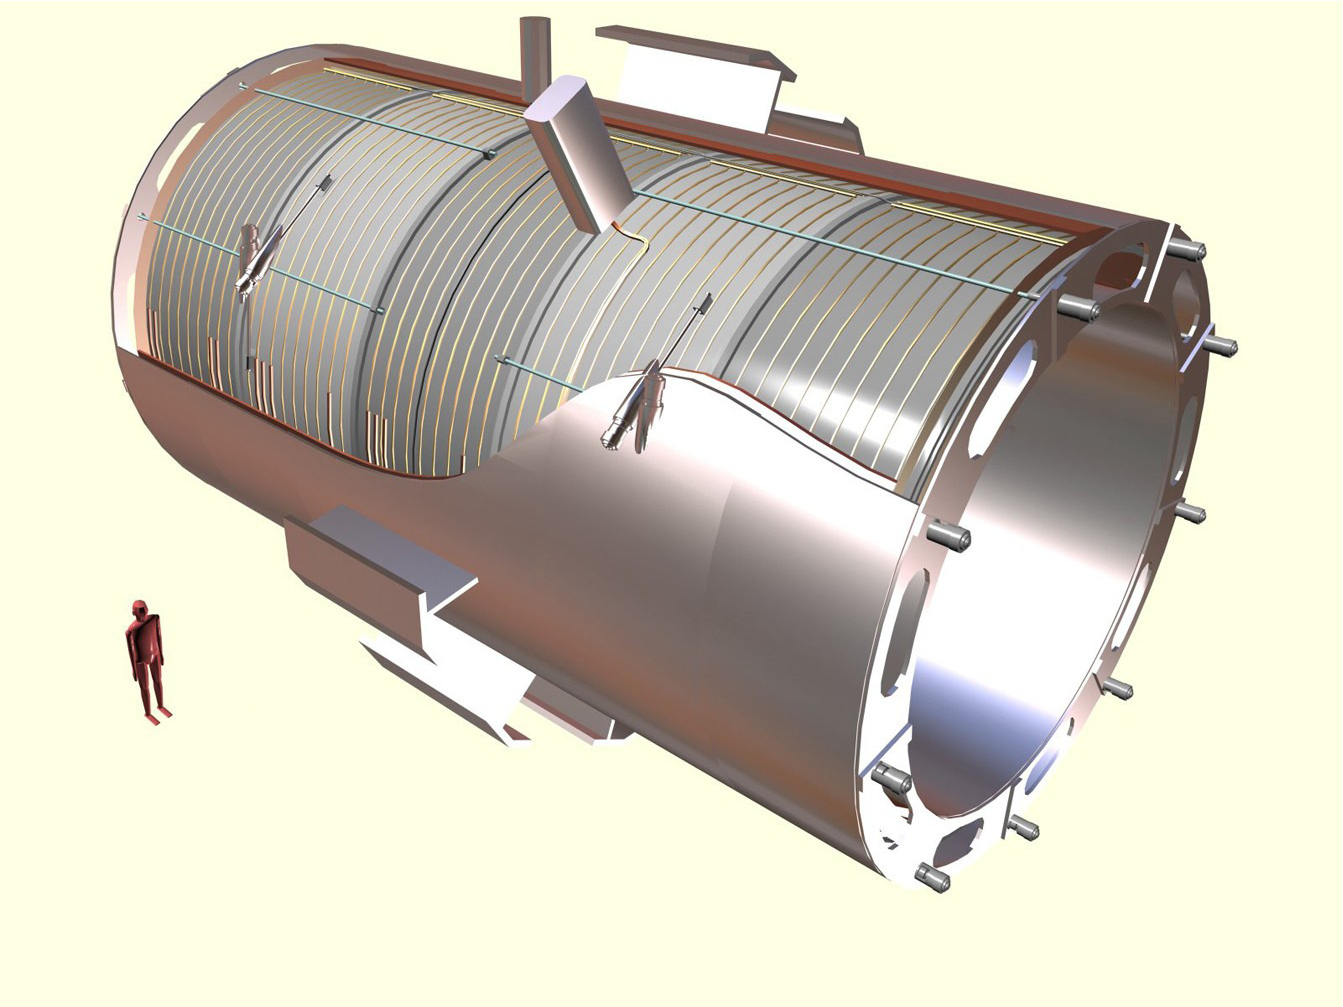
\includegraphics[width=0.75\textwidth]{ECALimages/magnet.png}
  	\caption[CMS Solenoid Magnet Layout]
   	{CMS Solenoid Magnet Layout}
	\label{fig:magnetLayout}
\end{figure}

The super conducting magnet consists of two main parts, the superconducting
solenoid and the return yoke.
Due to structural constraints, the solenoid itself is 6.3m in diameter and 12.5 m in length,
this is large enough to allow the tracker, electromagnetic calorimeter
and the hadronic calorimeter to be contained within the solenoid. This is
a desirable characteristic as it limits the number of radiation
lengths between the nominal collision point and these detectors. The solenoid
is composed of 4 layers of windings due to the large number of ampere-turns required
and is composed of NbTi. The windings and support structure of the solenoid
are detailed in Figure \ref{fig:magnetLayout}. 
The magnetic field is given by,
\begin{displaymath}
B=\mu_{0}nI
\end{displaymath}
where $\mu_{0}$ is the magnetic constant, n is the number of turns per unit length and 
I is the current. 
The flux is returned by a 10,000 ton yoke which is composed of 11 elements, 6 endcap disks 
and 5 barrel wheels. The yoke also was designed to contain four muon stations. 
Both the solenoid and the yoke also serve a dual purpose as a structural support 
for the CMS experiment. 